\documentclass[11pt,a4wide]{article}
\usepackage{verbatim}
\usepackage{listings}
\usepackage{graphicx}
\usepackage{a4wide}
\usepackage{color}
\usepackage{amsmath}
\usepackage{amssymb}
\usepackage[dvips]{epsfig}
\usepackage[T1]{fontenc}
\usepackage{cite} % [2,3,4] --> [2--4]
\usepackage{shadow}
\usepackage{hyperref}

\usepackage{subcaption}

\setcounter{tocdepth}{2}

\lstset{language=c++}
\lstset{alsolanguage=[90]Fortran}
\lstset{basicstyle=\small}
\lstset{backgroundcolor=\color{white}}
\lstset{frame=single}
\lstset{stringstyle=\ttfamily}
\lstset{keywordstyle=\color{red}\bfseries}
\lstset{commentstyle=\itshape\color{blue}}
\lstset{showspaces=false}
\lstset{showstringspaces=false}
\lstset{showtabs=false}
\lstset{breaklines}

\title{{\Huge {\bf Cool Title}}\linebreak \small{Project 2, FYS-3150}}
\author{Ina K. B. Kullmann}
\date{\today}

\begin{document}
\maketitle

\begin{center}
{ \scriptsize \noindent All source codes can be found at: \texttt{https://github.com/inakbk/Project\_2}. }
\end{center}

\tableofcontents
\newpage

\begin{abstract}
bla bla bla bla bla bla bla bla bla bla bla bla bla bla bla bla bla bla bla bla bla bla bla bla bla bla bla bla bla bla bla bla bla bla bla bla bla bla bla bla bla bla bla bla bla bla bla bla bla bla bla bla bla bla bla bla bla bla bla bla bla bla bla bla bla bla bla bla bla blav bla bla bla bla bla bla bla bla bla bla bla bla bla bla bla bla bla bla bla bla bla bla bla bla bla bla bla bla bla bla bla bla bla bla blav bla bla bla bla blav bla bla bla bla bla

bla bla bla bla bla bla bla bla bla bla bla bla bla bla bla bla bla bla bla bla bla bla bla bla bla bla bla bla bla bla bla bla bla bla bla bla bla bla bla bla bla bla bla bla bla bla bla bla bla bla bla bla bla bla bla bla bla bla bla bla bla bla bla bla bla bla bla bla bla blav bla bla bla bla bla bla bla bla bla bla bla bla bla bla bla bla bla bla bla bla bla bla bla bla bla bla bla bla bla bla bla bla bla bla blav bla bla bla bla blav bla bla bla bla bla
\end{abstract}


\section{Motivation and purpose}
The aim of this project is to solve Schr\"odinger's equation for two electrons in a three-dimensional harmonic oscillator well with and without a repulsive Coulomb interaction.  Your task is to solve this equation by reformulating it in a discretized form as an eigenvalue equation to be solved with Jacobi's method. -->code which implements Jacobi's method. --> plot the wave function for two electrons. first look at one electron, then two without coul and then with coul.

Electrons confined in small areas in semiconductors, so-called quantum dots, form a hot research area in modern solid-state physics, with applications spanning from such diverse fields as quantum nano-medicine to the contruction of quantum gates. You can read about quantum dots at \url{http://en.wikipedia.org/wiki/Quantum_dot}, which also contains links to several scientific articles. A recent article of interest is the review by Semonin {\em et al} in Materials Today, volume 15, page 508 (2012).

In this article we will let two electrons move in a three-dimensional harmonic oscillator potential that repel each other via the Coulomb interaction.  Throughout this paper we will assume spherically symmetry and let the angular momentum be $l=0$. Before solving the problem for two electrons we will look at one electron in a harmonic oscillator potential. 

To solve the Schr\"odinger's equation for one electron(and two??) we will have to transformed the equations into a matrix eigenvalue problem. When we have rewritten the problem we will use Jacobi's rotation algorithm to find the solutions. % (see Lecture notes chapter 7)   .

Together with linear equations and least squares, the third major problem in matrix com- putations deals with the algebraic eigenvalue problem. Here we limit our attention to the symmetric case. We focus in particular similarity transformations, --> Jacobi \footnote{sitert fra lectures2015 p. 225}


\newpage
\part{Theory}

\section{Numerical method}
\subsection{Solving eigenvalueproblems using similarity transformations}
%en av de over??
%(noe noe innledning)?? by using similarity transformations

Let us assume that we have the eigenvalue problem 
\[
\bf A \bf x^{(v)} = \lambda \bf x^{(v)}
\]
where $\lambda^{(v)}$ are the eigenvalues and $\bf x^{(v)}$ the corresponding eigenvectors.\footnote{The introduction to this section is based on the lecturenotes"lectures2015.pdf"} Assuming that the matrix $\bf A$ is real and symetric we can use the Jacobi rotation algoritm to solve the eigenvalue problem. First we will describe the use of similarity tansformations in general and then the Jacobi rotation algorithm in detail.

Let $\bf D$ be the diagonal matrix with the eigenvalues of $\bf A$ on the diagonal:

\begin{equation}
    \bf D = \left( \begin{array}{ccccccc} \lambda_1 & 0 & 0   & 0    & \dots  &0     & 0 \\
                                0  & \lambda_2 & 0 & 0    & \dots  &0     &0 \\
                                0   & 0 & \lambda_3 & 0  &0       &\dots & 0\\
                                \dots  & \dots & \dots & \dots  &\dots      &\dots & \dots\\
                                0   & \dots & \dots & \dots  &\dots       &\lambda_{n-1} & 0\\
                                0   & \dots & \dots & \dots  &\dots       &0 & \lambda_n

             \end{array} \right) 
      \label{eq:sematrix}
\end{equation} 

We say that a matrix $\bf B$ is a similarity transform of $\bf A$ if 
\[
\bf B = \bf {S^T AS}
\]
Where $\bf S$ is a unitary matrix so $\bf{S^TS} = \bf{S^{-1}S} = \bf I$. The point of this is that the matrix $\bf B$ has the same eigenvalues as $\bf A$. Since $\bf A$ is real and symetric there exists a real orthonogal matrix $\bf S'$ such that: %skjekk unitary i mat1120 boka?
\[
\bf {S'^T AS'} = \bf D
\]
So the strategy is then to perform a series of similarity transformations on the original matrix $\bf A$ so that the matrix reduces to the diagonal matrix $\bf D$ with the eigenvalues on the diagonal:
\[
\bf{S_N^T\dots S_1^TAS_1\dots S_N} = \bf D
\]
where $\bf{S_1\dots S_N} = \bf S'$. This must be done on both sides of the equation. Only one transformation is given by:
\begin{align*}
(\bf{S^TAS})(\bf{S^Tx}) = \lambda \bf{S^Tx} \\
\bf{B(S^Tx)} = \lambda\bf{(S^Tx)}
\end{align*}
using that $\bf S$ is unitary. We see that the eigenvalue of $\bf B$ is the same as for $\bf A$, but the eigenvector is changed to $\bf{S^Tx}$.

\subsection{Jacobi's rotation algorithm} \label{sec:jacobi}
We will now see how we can find the eigenvalues of a real and symetric matrix $\bf A$ by using the Jacobi's rotation algoritm, or Jacobi's method.

The Jacobi's method introduces the ($n\times n$) unitary orthogonal transformation matrix 
\begin{equation}
    \bf S = \left( \begin{array}{ccccccc} 1 & 0 & 0   & 0    & \dots  &0     & 0 \\
                                0  & 1 & 0 & 0    & \dots  &0     &0 \\
                                0   & 0 & \cos \theta & 0  &0       &\dots & \sin \theta\\
                                0   & 0 & 0  & 1  &0       &\dots & 0\\
                                \dots  & \dots & \dots & \dots  &\dots      &\dots & \dots\\
                                0   & \dots & \dots & \dots  &\dots       &1 & 0\\
                                0   & \dots & -\sin \theta & \dots  &\dots       &0 & \cos \theta

             \end{array} \right) 
      \label{eq:sematrix}
\end{equation}
that performs a plane rotation around an angle $\theta$ in the Euclidean $n$-dimensional space. For simpler notation we define the quantities $\tan\theta = t= s/c$, with $s=\sin\theta$ and $c=\cos\theta$. The elements of the matrix $\bf S$ that differ from zero is given by the indexes $k,l$:
\[
s_{kk} = s_{ll} = c, \;\;\;\;  s_{kl} = -s_{lk} = -s,\;\; \;\;  s_{ii} = 1
\]
where $i\neq k$, $i\neq l$ and $i,j$ are the indexes of the matrix. Then the similarity transformation 
\[
\bf B = \bf {S^T AS}
\]
can be written on component form as:
\begin{align*}
b_{ii} &= a_{ii}\\
b_{ik} &= ca_{ik} - sa_{il} \\
b_{il} &= ca_{il} - sa_{ik} \\
b_{kk} &= c^2a_{kk} - s csa_{kl} + s^2 a_{ll} \\
b_{ll} &= c^2a_{ll} + 2csa_{kl} + s^2a_{kk} \\
b_{kl} &= cs(a_{kk} - a_{ll}) + (c^2 - s^2)a_{kl}
\end{align*}
We want to choose the angle $\theta$ so that all the non-diagonal matric elements becomes zero, that is $b_{kl} = 0$. Introducing a new variable $\tau$ dependent on $k,l$:
\begin{align*}
b_{kl} &= cs(a_{kk} - a_{ll}) + (c^2 - s^2)a_{kl} = 0\\
&\Rightarrow \frac{a_{ll}-a_{kk}}{a_{kl}} = \frac{c^2 - s^2}{cs} = \frac{2\cos{2\theta}}{\sin{2\theta}} = 2 \cot{2\theta}\\
&\Rightarrow \tau = \cot{2\theta} = \frac{a_{ll}-a_{kk}}{2a_{kl}}
\end{align*}
Then $b_{kl} = 0$ can be written as a second order equation
\begin{align*}
2\tau &= \frac{c^2 - s^2}{cs} = \frac{c^2}{cs} - \frac{s^2}{cs} = \frac{1}{t} - t\\
&\Rightarrow 2\tau t = 1 - t^2 \\
&\Rightarrow t^2 +2\tau t - 1 = 0\\
\end{align*}
with the solution
\[
t = -\tau \pm\sqrt{1 + \tau^2}.
\]
We obtain $c$ ans $s$ from
\begin{align*}
c^2 + s^2 = 1\\
\Rightarrow c = \frac{1}{\sqrt{1+t^2}},
\end{align*}
and using that $s=tc$.  

But which of the roots of $t$ should we choose? To make shure that the the similarity transformation does not make bigger changes to the other elements of $\bf A$ while making another element zero we minimize the difference between the matrices ${\bf B}$ and ${\bf A}$ by letting  $|\theta| \leq \pi /4$. This also makes shure that the iterations goes faster toward the solution, else the iterations might not converge at all after a reasonable number of iterations. 

Separating the inequality gives $\theta \leq \pi/4$ and $\theta \geq -\pi/4$. Starting with the first inequality:
\begin{align*}
\theta = \arctan t &\leq \pi/4 \\
t &\leq \tan (\pi/4) = 1
\end{align*}
and 
\begin{align*}
\theta = \arctan t &\geq -\pi/4 \\
t &\geq \tan(-\pi/4) = -1
\end{align*}
so we see that $|t| \leq 1\Rightarrow -\tau \pm \sqrt{1 + \tau^2} \leq 1$. If we look at the case where $\tau > 0$ and try the positive root of $t$ we see that:
\begin{align*}
-\tau + \sqrt{1 + \tau^2} &\leq -|\tau| + 1 + |\tau| = 1 \\
&\Rightarrow t \leq 1 \Rightarrow \theta \leq \pi/4
\end{align*}
must be satisfied.

If we then try the case when $\tau < 0$ and the negative root of $t$ we see that:
\begin{align*}
-\tau - \sqrt{1 + \tau^2} &= |\tau| - \sqrt{1 + \tau^2} \geq |\tau| - (1 + |\tau|) = -1 \\
&\Rightarrow t \geq -1 \Rightarrow \theta \geq -\pi/4
\end{align*}
must be satisfied. So the choice of the root of $t$ is dependent on $\tau$. When $\tau > 0$ we choose the positive root, and when $\tau< 0$ we choose the negative root to make shure that $|\theta| \leq \pi /4 $ is satisfied. \\~\\

The Jacobi algorithm can then be described as follows: 
\begin{enumerate}
\item Find the indexes $k, l$ of the maximum element of the matrix $\bf A$.
\item Obtain $c$ and $s$, the matrix elements of $\bf S$, given by $k, l$.
\item Calculate the similarity transformation $\bf{B = S^TAS}$.
\item Start on [1.] again, setting $\bf {A = B}$, untill all off-diagonal elements are esentially zero (less than a given threshold). When the iterations stop the eigenvalues are given by the matrix $\bf {D = B}$.
\end{enumerate}

We see that all information needed to perform a Jacobi rotation is given by the indexes $k, l$ of the maximum elements of $\bf A$.

\subsubsection*{Retriving the eigenvectors}
In this particular problem we also want to find the eigenvectors $\bf x^{(v)}$ of the matrix $\bf A$. The Jacobi's rotation method described in section \ref{sec:jacobi} does not return the eigenvectors. For every similarity transformation in the Jacobi's method the eigenvector is changed from $\bf x$ to $\bf{S^Tx}$. So it is possible to add a routine to the Jacobi's algorithm which ceeps track of the changes to the eigenvectors so that the eigenvectors can be returned when the iterations stop. This is a bit tricy and the eigenvectors also need to be normalized.

We will use the existing {\em tqli} function found at(??). Here the eigenvectors are obtained from the matrix $z[i][j]$, where the index $j$ refers to eigenvalue $j$. The index $i$ points to the value of the wave function in position $\rho_j$. That is,  $u^{(\lambda_j)}(\rho_i)=z[i][j]$.   

The eigenvectors are normalized. 

(change this one!)

\section{A simple system: One electron in a three-dimensional harmonic oscillator potential.}
here we will look eqiation (?)

A system with known solutions, good for testing
\subsection{Rewriting the Schr\"odinger's equation to a dimensionless form} \label{sec:rewrite_sch}
We look at the Sch\"odinger's equation for one electron at a radius $r\in [0,\infty)$ in a harmonic oscillator potential given by: 
\[
V(r)= (1/2)kr^2
\]
where $k=m\omega^2$ and $\omega$ is the oscillator frequence. The energy $E$ of the harmonic oscillator in three dimensions is given by:
\[
E_{nl}=  \hbar \omega \left(2n+l+\frac{3}{2}\right),
\]
with $n=0,1,2,\dots$ and $l=0,1,2,\dots$ is the orbital momentum of the electron. 

We are only interested in the solution of the radial part of the Schr\"odinger equation given by
\begin{equation}
  -\frac{\hbar^2}{2 m} \left ( \frac{1}{r^2} \frac{d}{dr} r^2
  \frac{d}{dr} - \frac{l (l + 1)}{r^2} \right )R(r) 
     + V(r) R(r) = E R(r).
     \label{eq:schr_1}
\end{equation}

We then use the substitution $R(r) = (1/r) u(r)$ and obtain
\[
  -\frac{\hbar^2}{2 m} \frac{d^2}{dr^2} u(r) 
       + \left ( V(r) + \frac{l (l + 1)}{r^2}\frac{\hbar^2}{2 m}
                                    \right ) u(r)  = E u(r) .
\]
The boundary conditions are $u(0)=0$ and $u(\infty)=0$.

We will modify equation \ref{eq:schr_1} further by introducing a dimensionless variable $\rho = (1/\alpha) r$ where $\alpha$ is a constant with dimension length and get
% 
\[
  -\frac{\hbar^2}{2 m \alpha^2} \frac{d^2}{d\rho^2} u(\rho) 
       + \left ( V(\rho) + \frac{l (l + 1)}{\rho^2}
         \frac{\hbar^2}{2 m\alpha^2} \right ) u(\rho)  = E u(\rho) .
\]
%
Now inserting $l=0$ and the rewritten potential $V(\rho) = (1/2) k \alpha^2\rho^2$ we obtain:
\[
  -\frac{\hbar^2}{2 m \alpha^2} \frac{d^2}{d\rho^2} u(\rho) 
       + \frac{k}{2} \alpha^2\rho^2u(\rho)  = E u(\rho) .
\]
and then multiply by $2m\alpha^2/\hbar^2$ on both sides
\[
  -\frac{d^2}{d\rho^2} u(\rho) 
       + \frac{mk}{\hbar^2} \alpha^4\rho^2u(\rho)  = \frac{2m\alpha^2}{\hbar^2}E u(\rho) .
\]
We fix the constant $\alpha$ so that
\[
\frac{mk}{\hbar^2} \alpha^4 = 1 \Rightarrow \alpha = \left(\frac{\hbar^2}{mk}\right)^{1/4}.
\]
and then define 
\[
\lambda = \frac{2m\alpha^2}{\hbar^2}E,
\]
Finally equation \ref{eq:schr_1} can be written as
\begin{equation}
  -\frac{d^2}{d\rho^2} u(\rho) + \rho^2u(\rho)  = \lambda u(\rho) .
  \label{eq: sch_1D_final}
\end{equation}
which is the equation we want to solve numerically. We know\footnote{This is given in the assignment text for Project 2, FYS3150..} that this equation has the eigenvalues $\lambda_0=3,\lambda_1=7,\lambda_2=11,\dots .$ for $l=0$. These analytical values will be used compare with the numerical solution in this one electron system.

\subsection{Discretizing the Schr\"odingers equation to solve the equation numerically.} \label{sec: descrete}
We will now rewrite the Schr\"odingers equation on a discretized form to be able to solve it as an matrix eigenvalue problem.

We use the expression for the second derivative of the function $u(\rho)$
\begin{equation}
    u''=\frac{u(\rho+h) -2u(\rho) +u(\rho-h)}{h^2} +O(h^2),
    \label{eq:diffoperation}
\end{equation} 
where $h$ is our step. We define the minimum and maximum values for the variable $\rho$,
$\rho_{\mathrm{min}}=0$  and $\rho_{\mathrm{max}}$ so that:
\[
  h=\frac{\rho_{\mathrm{max}}-\rho_{\mathrm{min}} }{n_{\mathrm{step}}}.
\]
where $n_{\mathrm{step}}$ is a given number of steps. Since $\rho \propto r$ and $r\in [0,\infty)$ the maximum value of $\rho$ should be $\rho_{\mathrm{max}}=\infty$. But we cannot set a infinite value when computing the solution numerically. We will therefore have to choose a significally large enough $\rho$.

We can then define an arbitrary value of $\rho$ as 
\[
    \rho_i= \rho_{\mathrm{min}} + ih \hspace{1cm} i=0,1,2,\dots , n_{\mathrm{step}}
\]
so that the Schr\"odinger equation for $\rho_i$ reads
\[
-\frac{u(\rho_i+h) -2u(\rho_i) +u(\rho_i-h)}{h^2}+\rho_i^2u(\rho_i)  = \lambda u(\rho_i),
\]
or in a more compact way with the harmonic oscillator potential $V_i=\rho_i^2$:
\begin{equation}
-\frac{u_{i+1} -2u_i +u_{i-1} }{h^2}+V_iu_i  = \lambda u_i,
\label{eq: sch_discrete_first}
\end{equation}
Then we can define first the diagonal matrix element
\[
   d_i=\frac{2}{h^2}+V_i,
\]
and the non-diagonal matrix element:
\[
   e_i=-\frac{1}{h^2}.
\]
We observe that in this case all the non-diagonal matrix element is given by a constant, so we can denote them all as $e=-\frac{1}{h^2}$ instead. (insert e og ikke ei hele veien??)
 
With these definitions the Schr\"odinger equation (\ref{eq: sch_1D_final}) takes the following form
\begin{equation}
d_iu_i+e_{i-1}u_{i-1}+e_{i+1}u_{i+1}  = \lambda u_i,
\label{eq: sch_1d_descrete}
\end{equation}
where $u_i$ is unknown. This can be written as a matrix eigenvalue problem
\begin{equation}
    \left( \begin{array}{ccccccc} d_1 & e_1 & 0   & 0    & \dots  &0     & 0 \\
                                e_1 & d_2 & e_2 & 0    & \dots  &0     &0 \\
                                0   & e_2 & d_3 & e_3  &0       &\dots & 0\\
                                \dots  & \dots & \dots & \dots  &\dots      &\dots & \dots\\
                                0   & \dots & \dots & \dots  &\dots       &d_{n_{\mathrm{step}}-2} & e_{n_{\mathrm{step}}-1}\\
                                0   & \dots & \dots & \dots  &\dots       &e_{n_{\mathrm{step}}-1} & d_{n_{\mathrm{step}}-1}

             \end{array} \right)      \left( \begin{array}{c} u_{1} \\
                                                              u_{2} \\
                                                              \dots\\ \dots\\ \dots\\
                                                              u_{n_{\mathrm{step}}-1}
             \end{array} \right)=\lambda \left( \begin{array}{c} u_{1} \\
                                                              u_{2} \\
                                                              \dots\\ \dots\\ \dots\\
                                                              u_{n_{\mathrm{step}}-1}
             \end{array} \right) 
      \label{eq:sematrix}
\end{equation} 
This is the final equation that we will solve numerically. We will test the implementation of the problem by comparing with the analytical eigenvalues, but we are also interested in the eigenvector of the ground state so that we can plot the probability distrubution.

\section{A complex system: Two electrons in a three-dimensional harmonic oscillator potential with Coulomb interaction.}
We will now study two electrons in a harmonic oscillator well which also interact via a repulsive Coulomb interaction.


We will now rewrite the single-electron equation as
\[
  -\frac{\hbar^2}{2 m} \frac{d^2}{dr^2} u(r) 
       + \frac{1}{2}k r^2u(r)  = E^{(1)} u(r),
\]
where $E^{(1)}$ stands for the energy with one electron only.

look at with and without Coulom
again we only interested in the ground state with $l=0$. 


\subsection{The two electron system without Coulomb interaction}
The Schr\"odingers equation for two electrons in a harmonic oscillator potential with no Coulomb interaction can be written as
\begin{equation}
\left(  -\frac{\hbar^2}{2 m} \frac{d^2}{dr_1^2} -\frac{\hbar^2}{2 m} \frac{d^2}{dr_2^2}+ \frac{1}{2}k r_1^2+ \frac{1}{2}k r_2^2\right)u(r_1,r_2)  = E^{(2)} u(r_1,r_2) 
\label{eq: sch_2d_uC}
\end{equation}
with a two-electron wave function $u(r_1,r_2)$ and the two-electron energy $E^{(2)}$.

Since there is no electron interaction equation \ref{eq: sch_2d_uC} is separabel, it can be written as the product of two single-electron wave functions. We introduce the relative coordinate ${\bf r} = {\bf r}_1-{\bf r}_2$ and the center-of-mass coordinate ${\bf R} = 1/2({\bf r}_1+{\bf r}_2)$. With these new coordinates,  equation \ref{eq: sch_2d_uC} reads
\[
\left(  -\frac{\hbar^2}{m} \frac{d^2}{dr^2} -\frac{\hbar^2}{4 m} \frac{d^2}{dR^2}+ \frac{1}{4} k r^2+  kR^2\right)u(r,R)  = E^{(2)} u(r,R).
\]

We can separate this equation into equations for $r$ and $R$ since the wave function $u(r,R) = \psi(r)\phi(R)$ is a product. The energy is given by the sum of the relative energy $E_r$ and the center-of-mass energy $E_R$, that is
\[
E^{(2)}=E_r+E_R.
\]
For this article we will omit the center-of-mass energy in the calculations. Then the equation of interest becomes:
\[
\left(  -\frac{\hbar^2}{m} \frac{d^2}{dr^2}+ \frac{1}{4}k r^2\right)\psi(r)  = E_r \psi(r).
\]
By following the same approach as in section \ref{sec: descrete} equation \ref{eq: sch_2e_wCol} can written on a dimensionless form as:
\[
\left(  - \frac{d^2}{d\rho^2}+ \frac{1}{\rho}\right)\psi(\rho)  = \lambda\psi(\rho).
\]
We can then use equation \ref{eq:sematrix} to solve the problem numerically if the potential is replaced:
\[
V_i = \rho^2 \rightarrow V_i = \frac{1}{\rho}
\]
We will plot the probability distrubution to see if the results are reasonable before implementing the Coulumb interaction.

\subsection{The two electron system with Coulomb interaction}
We will now include the repulsive Coulomb interaction between two electrons. Introducing the term
\[
V(r_1,r_2) = \frac{\beta e^2}{|{\bf r}_1-{\bf r}_2|}=\frac{\beta e^2}{r},
\]
with $\beta e^2=1.44$ eVnm. With this extra term representing the interaction the $r$-dependent Schr\"odinger equation becomes
\[
\left(  -\frac{\hbar^2}{m} \frac{d^2}{dr^2}+ \frac{1}{4}k r^2+\frac{\beta e^2}{r}\right)\psi(r)  = E_r \psi(r).
\]

We want to manipulate this equation further to make it as similar as possible to the one electron equation (\ref{eq:schr_1}) we obtained earlier. Again we introduce the dimensionless variable $\rho = r/\alpha$ and repeating the same steps as in section \ref{sec:rewrite_sch}, we arrive at 
\[
  -\frac{d^2}{d\rho^2} \psi(\rho) 
       + \frac{1}{4}\frac{mk}{\hbar^2} \alpha^4\rho^2\psi(\rho)+\frac{m\alpha \beta e^2}{\rho\hbar^2}\psi(\rho)  = 
\frac{m\alpha^2}{\hbar^2}E_r \psi(\rho) .
\]
We manipulate this equation further by defining a 'frequency' which reflects the strength of the oscillator potential
\[
\omega_r^2=\frac{1}{4}\frac{mk}{\hbar^2} \alpha^4,
\]
and fix the constant $\alpha$ by requiring 
\[
\frac{m\alpha \beta e^2}{\hbar^2}=1
\]
or 
\[
\alpha = \frac{\hbar^2}{m\beta e^2}.
\]
Then defining 
\[
\lambda = \frac{m\alpha^2}{\hbar^2}E,
\]
so we finally can write the Schr\"odinger's equation as
\begin{equation}
  -\frac{d^2}{d\rho^2} \psi(\rho) + \omega_r^2\rho^2\psi(\rho) +\frac{1}{\rho} = \lambda \psi(\rho).
  \label{eq: sch_2e_wCol}
\end{equation}
We can again use equation \ref{eq:sematrix} to solve the problem numerically if the potential is replaced:
\[
V_i = \rho^2 \rightarrow V_i = w_r^2\rho^2 + \frac{1}{\rho}
\]

For specific oscillator frequencies, the above equation has answers in an analytical form found by M.~Taut\footnote{M.~Taut, Phys. Rev. A 48, 3561 - 3566 (1993).The article can be retrieved from the following web address \url{http://prola.aps.org/abstract/PRA/v48/i5/p3561_1}}. We will plot the probability distrubution for the cases $\omega_r = 0.01$, $\omega_r = 0.5$, $\omega_r =1$, and $\omega_r = 5$ for the ground state only ($l=0$).




\newpage
\part{Implementation, testing and finding the solutions of the Schr\"odinger equations}

\section{Implementation and testing of the Jacobi algorithm} \label{sec: test_jacobi}
\subsubsection*{Implementation}
The Jacobi rotation algorithm is structured into separate files which can be run once from \texttt{main.cpp} to solve one eigenvalueproblem. All files refered to in this section can be found in the folder \texttt{project\_2\_test\_jacobi} at: \\
\texttt{https://github.com/inakbk/Project\_2/tree/master/project\_2\_test\_jacobi}

The \texttt{jacobi.h} file contains all the routines for one rotation. The code finds the maximum element of the matrix, obtains the transformation matrix and does one rotation. The \texttt{jacobisolver.h} file does all the rotations for a given matrix $\bf B$ by calling the \texttt{jacobi.h} code and returns the eigenvalues and the first eigenvector. The parameter \texttt{tolerance} sets the limit of how small all the off diagonal elements in the matrix $\bf B$ needs to be before the rotations stop and the eigenvalues and the first eigenvector are returned. If the number of rotations (\texttt{numberOfIterations}) exceeds the maximum number of rotations (\texttt{maxNumberOfIterations}) before the off diagonal elements are smaller than the tolerance, the opreations are aborted with a warning message that the routine did not converge. The code also computes the execution time of all iterations for one matrix. 

We then see that the code in \texttt{jacobisolver.h} does the whole job of solving the eigenvalue problem with the Jacobi method and need only be given the matrix $\bf B$ with its dimension and the maximum number of iterations. Then the \texttt{main.cpp} program only needs to constructs the matrix $\bf B$ and call the \texttt{jacobisolver.h} code. With the help of \texttt{writetofile.h} the main program will write all parameters and the eigenvalues and eigenvectors to a file with filenames that distinguish the parameters that where run. These datafiles will then later be read by a python script and plot the data. 

\subsubsection*{Testing of the code}
Before using the Jacobi algorithm solve the physical problems the code was tested to make sure it worked properly. The purpose of the files in the folder \texttt{project\_2\_test\_jacobi} is to test the implementation of the Jacobi algorithm.

To do this the matrix $\bf B$ is initialized to a random symetric matrix. Then the solution is compared to the solutions generated by the \texttt{eig\_sym} function in the armadillo library.

To initialize $\bf B$ as a symetrix matrix we let $\bf C$ be a random matrix and set $\bf B = \bf{CC^T}$. Then $\bf B$ is a symetric matrix:
\[
\bf { B^T = (CC^T)^T = (C^T)^TC^T = CC^T = B}
\]
using that $\bf{ (ab)^T = b^Ta}$\footnote{\texttt{https://en.wikipedia.org/wiki/Transpose} (I dont have the mat1120 book here so wikipedia refrences it is then..)}. 

\section{Using the Jacobi rotation algorithm to solve the Schr\"odinger equations}

Equation \ref{eq:sematrix} is the matrix equation that we can use to solve both the one and two electron systems. The only difference between the systems are the potential $V_i$ and hence the matrix $\bf B$.

We can solve equation \ref{eq:sematrix} numerically using the Jacobi rotation algorithm as described in section \ref{sec: test_jacobi} by using the files \texttt{jacobisolver.h} and \texttt{jacobi.h} and \texttt{writetofile.h} to save the results. But in \texttt{main.cpp} the matrix would have to be initialized to the matrix in equation \ref{eq:sematrix}:
\[
\bf B = \left( \begin{array}{ccccccc} d_1 & e & 0   & 0    & \dots  &0     & 0 \\
                                e & d_2 & e & 0    & \dots  &0     &0 \\
                                0   & e & d_3 & e  &0       &\dots & 0\\
                                \dots  & \dots & \dots & \dots  &\dots      &\dots & \dots\\
                                0   & \dots & \dots & \dots  &\dots       &d_{n_{\mathrm{step}}-2} & e\\
                                0   & \dots & \dots & \dots  &\dots       &e & d_{n_{\mathrm{step}}-1}

             \end{array} \right)
\]
This is done in the folders \texttt{project\_2\_1e}, \texttt{project\_2\_2e} and \texttt{project\_2\_2e\_w\_col}\footnote{The reason the folders are separated are to not mix up the result files and be shure to be able to reproduce the results and look back if something is strange at a later point.} for respectively the one electron system and the two electron system without Coulomb interaction and with Coulumb interaction. The only difference between the folders are the potentials, or the matrix $\bf B$, the \texttt{.h} files are identical. The only exception is that the parameter $w_r$ is included in the last two electron case. 

But before the Schr\"odinger equations can be solved numerically the value of $p_{\mathrm{max}}$ and $n_{\mathrm{step}}$ that we will use needs to be decided.  

\subsection{Finding reasonable values for $p_{\mathrm{max}}$ and $n_{\mathrm{step}}$}

The matrix $\bf B$ is only dependent on the elements $d_i$ and $e$ which is only dependent on $p_{\mathrm{max}}$ and the dimension of the matrix $n_{\mathrm{step}}$. So which values of $p_{\mathrm{max}}$ and $n_{\mathrm{step}}$ should we choose? We need to test the algorithm so that we know which $p_{\mathrm{max}}$ that gives stable results and which values of $n_{\mathrm{step}}$ it is reasonable to use. 

First we have to decide which $p_{\mathrm{max}}$ to choose as this might affect the choice of $n_{\mathrm{step}}$. This can be done by looking at the first eigenvalues and choose the $p_{\mathrm{max}}$ which gives the smallest error when comparing to the analytical values. For the two electron case there are no analytical values to compare with so it is reasonable to choose a value which gives the most stable eigenvalues as a finction of  $n_{\mathrm{step}}$. We will therefore plot the eigenvalues as a function of $p_{\mathrm{max}}$.

Then we have to decide which precition of the eigenvalues we want to set a limit on how large $n_{\mathrm{step}}$ needs to be. This can be done by choosing a value of $n_{\mathrm{step}}$ that gives a small enough absolute error in the first three eigenvalues and that also have a reasonable execution time. We will plot the absolute error in the eigenvalues as a function of $n_{\mathrm{step}}$ to investigate this.

The execution time and precition is also related to how close to zero we force the off diagonal elements of $\bf B$ to be before reading off the eigenvalues. If the tolerance is too low we end up doing a lot of extra rotations that are very time consuming. We therefore should choose a tolerance that is low enough, but not too small. The number of transformations and the execution time will also be plotted as a function of $n_{\mathrm{step}}$.

When we are done deciding on the values of $p_{\mathrm{max}}$ and $n_{\mathrm{step}}$ the the Schr\"odinger equations can be solved numerically as described in the beginning of this section. 



\newpage
\part{Results and discussion}
%\subsection*{Choice of $p_{\mathrm{max}}$ }

All this is for 1e:

Figure \ref{fig: p_max_big} example normal, goes to zero

\begin{figure} [ht]
\centering
\includegraphics[width=0.7\textwidth]{plots_1e/p_max_n100_big.png}
\caption{noe langt}
\label{fig: p_max_big}
\end{figure}

Figure \ref{fig: p_max_zoom} see 4 diff n and choice
\begin{figure} [t!]
\centering
	\begin{subfigure}[t]{0.7\textwidth}
		\centering
		\includegraphics[width=1\textwidth]{plots_1e/p_max_n50_z.png}
		\includegraphics[width=1\textwidth]{plots_1e/p_max_n100_z.png}
		%\caption{noe langt om langt}
	\end{subfigure}
	~
	\begin{subfigure}[t]{0.7\textwidth}
		\centering
		\includegraphics[width=1\textwidth]{plots_1e/p_max_n150_z.png}
		\includegraphics[width=1\textwidth]{plots_1e/p_max_n200_z.png}
		%\caption{noe langt om langt2}
	\end{subfigure}
\caption{noenoe langt}
\label{fig: p_max_zoom}
\end{figure}

in fig \ref{fig: abs.err_n} see error plotted against n
\begin{figure} [ht]
\centering
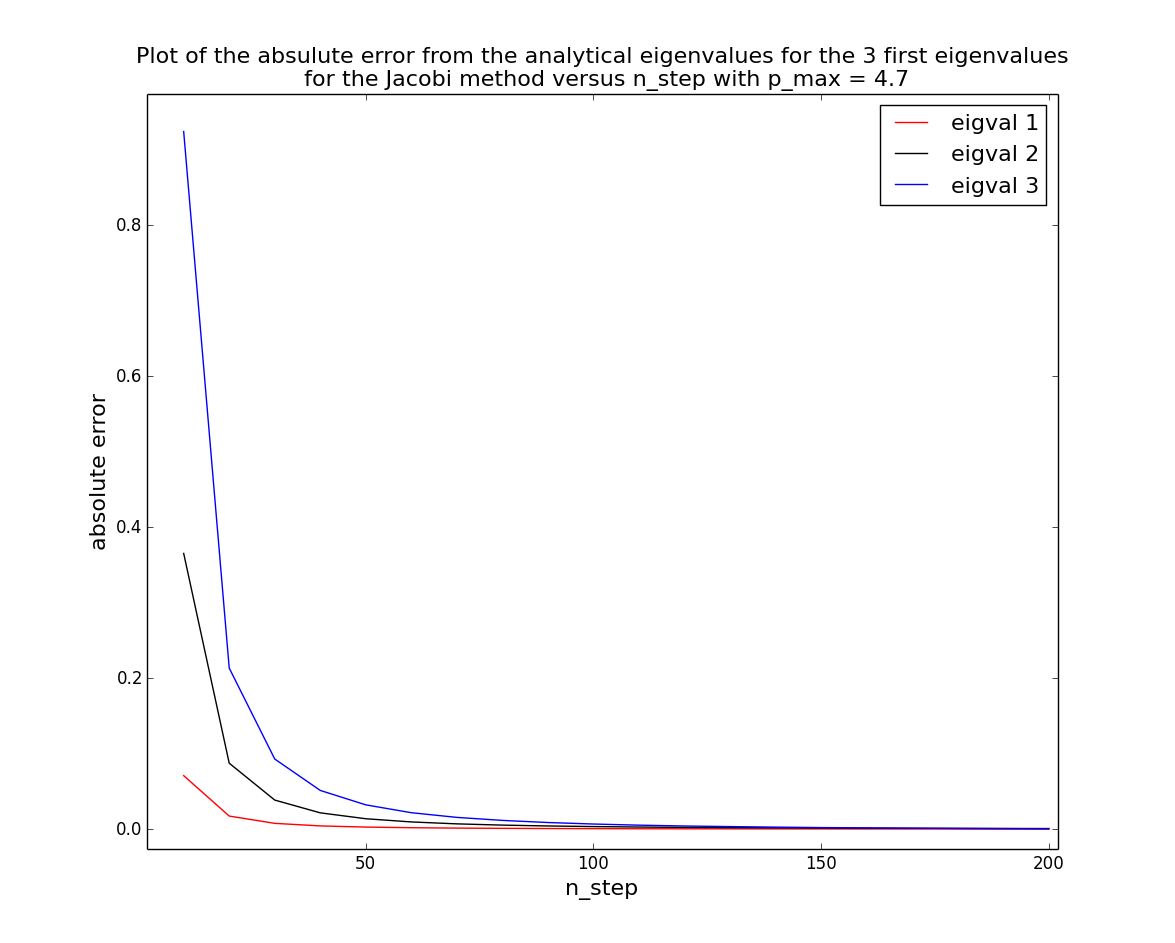
\includegraphics[width=0.7\textwidth]{plots_1e/abs_error.png}
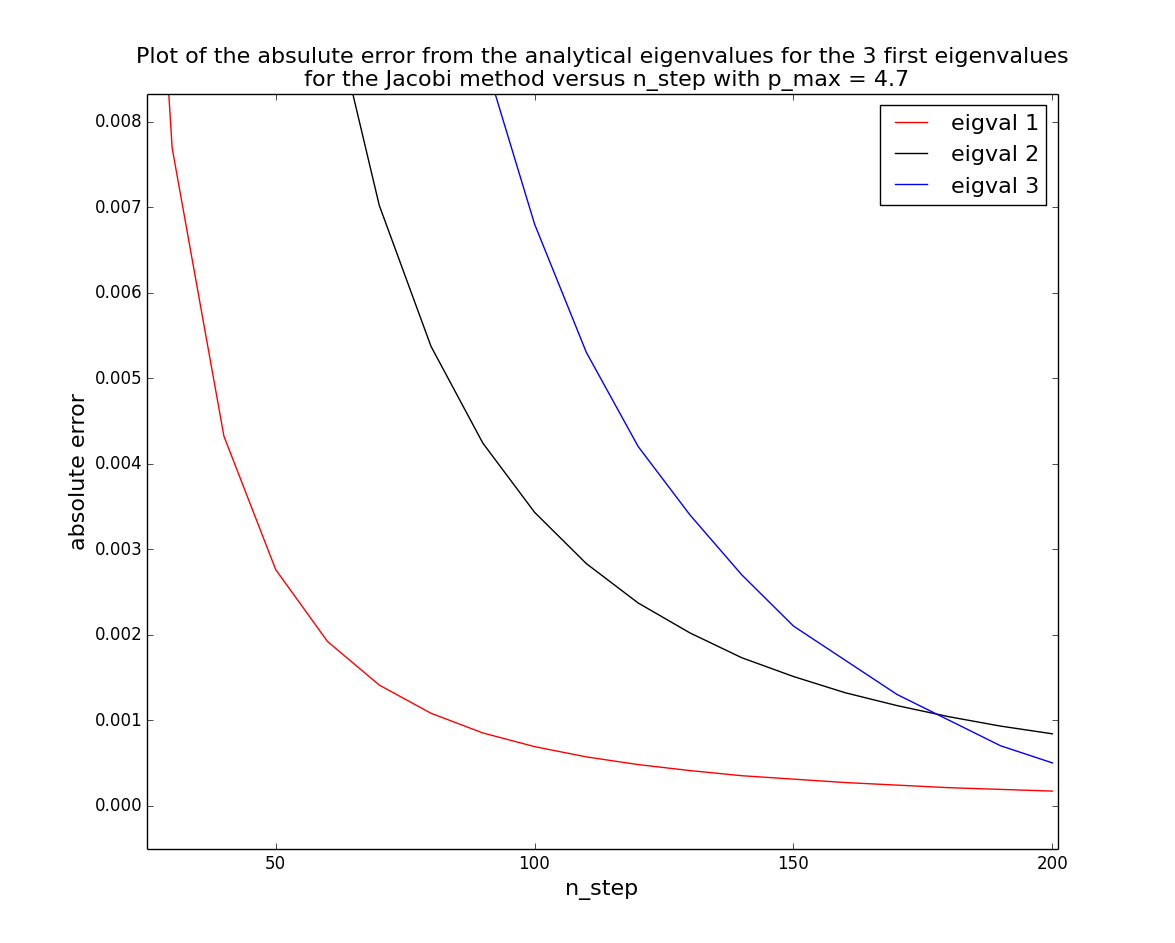
\includegraphics[width=0.7\textwidth]{plots_1e/abs_error_zoom.png}
\caption{noe langt}
\label{fig: abs.err_n}
\end{figure}

in fig \ref{fig: nr_iter} see nr iter vs n
\begin{figure} [ht]
\centering
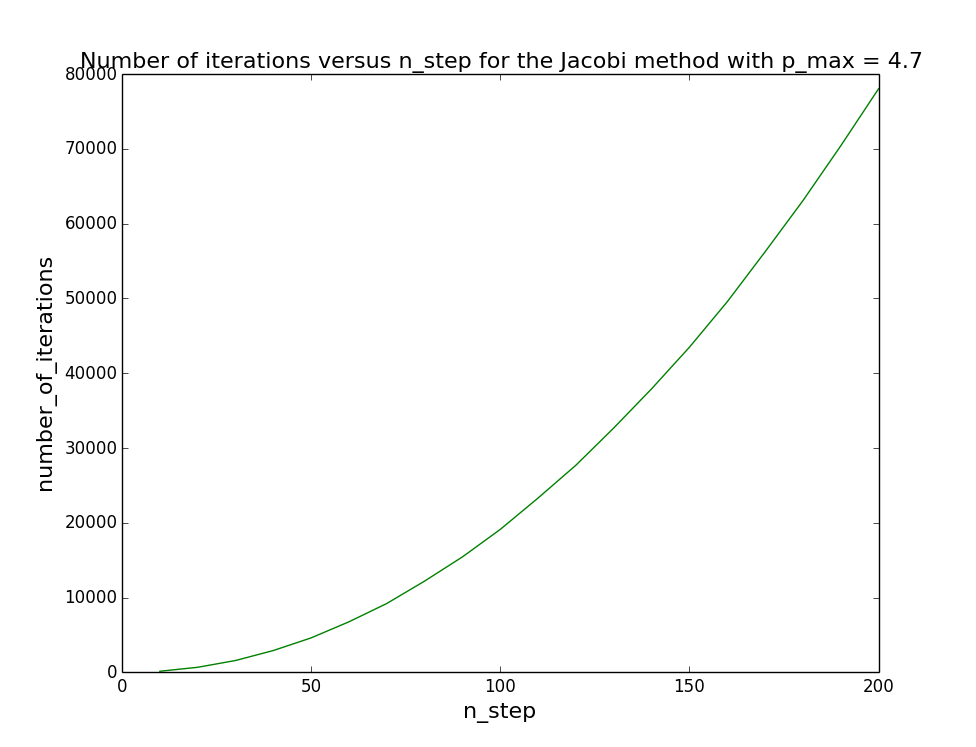
\includegraphics[width=0.7\textwidth]{plots_1e/nr_iterations.png}
\caption{noe langt}
\label{fig: nr_iter}
\end{figure}

in fig \ref{fig: nr_iter} see time vs n

\begin{figure} [ht]
\centering
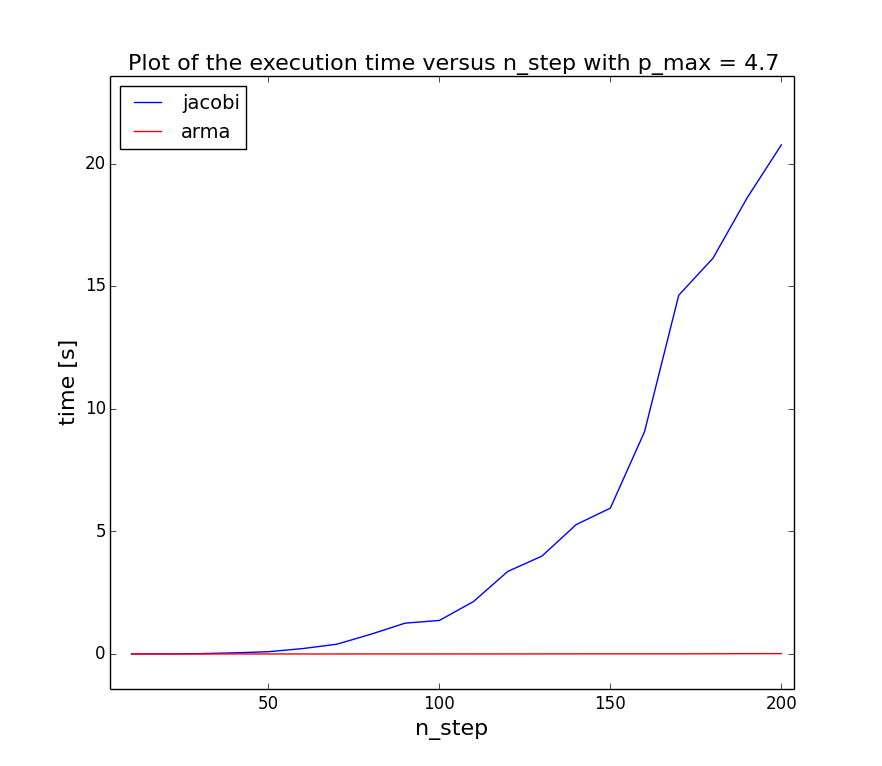
\includegraphics[width=0.7\textwidth]{plots_1e/time.png}
\caption{noe langt}
\label{fig: nr_iter}
\end{figure}

\noindent\rule{\textwidth}{1pt}
With no repulsive Coulomb interaction 
you should get a result which corresponds to 
the relative energy of a non-interacting system.   
Make sure your results are 
stable as functions of $\rho_{\mathrm{max}}$ and the number of steps.
\noindent\rule{\textwidth}{1pt}

\noindent\rule{\textwidth}{1pt}
Comment the results for the lowest state (ground state) as function of
varying strengths of $\omega_r$. 
\noindent\rule{\textwidth}{1pt}




\noindent\rule{\textwidth}{1pt} 
Here you are asked to implement unit tests in your C++ program. For C++ users, please follow the guidelines on how to install unit tests with c++ on the webpage. These issues will be discussed in more detail at the lab and lectures during week 38. 




\end{document}





